\documentclass{beamer}
\usepackage{lmodern}
\usepackage[frenchb]{babel}
\usepackage[T1]{fontenc}
\usepackage[utf8]{inputenc}
\usepackage{amsmath}

\usetheme{Warsaw}

\title{Maximum Probability Shortest Path Problem}
\author{Jeremy Krebs - Guillaume Soulié}
\institute{Université Paris Saclay}
\date{\today}

\addtobeamertemplate{navigation symbols}{}{%
    \usebeamerfont{footline}%
    \usebeamercolor[fg]{footline}%
    \hspace{1em}%
    \insertframenumber/\inserttotalframenumber
}

\begin{document}

\begin{frame}
\titlepage
\end{frame}

% --------- Sommaire ---------
\begin{frame}
  \tableofcontents
\end{frame}      
% ----------------------------

\begin{frame}
Shortest Path is a known problem and has many applications in "real life".

\begin{itemize}
	\item Goods transport (industrial and private)
	\item Food Delivery (Deliveroo - Foodora - UberEats)
\end{itemize}

\end{frame}

\section{State of the art}

\begin{frame}

As this problem is well known, lots of scientists presented their work on related subject, most of the times with different hypotheses:

\begin{itemize}
	\item<2-> Without resource constraints
	\item<3-> With deterministic resource constraints
	\item<4-> With stochastic resource constraints
\end{itemize}

\uncover<5->{or also with a different optimization problem like utility functions to maximize or cost functions to minimize.}
\end{frame}

\section{Problem}
\subsection{Description}

\begin{frame}
	<Insert Picture from the article and explain orally>
\end{frame}

\subsection{Hypothesis}
\begin{frame}
	\begin{itemize}
		\item Graph with weights on arcs, source node $s$ and sink node $t$,
		\item Stochastic resource consumptions with normal distribution,
		\item K resources,
		\item Threshold C of the cost function (maximum allowed weight of the path).
	\end{itemize}
	\pause
	\hspace*{-1.5cm}
	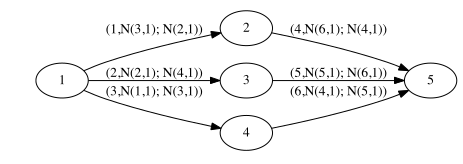
\includegraphics[width=12cm]{media/SRCSP_2.png}
\end{frame}

\subsection{Formulation}
\begin{frame}

SRCSP can be formulated as this optimization problem:

\begin{align*}
 max\ &\mathbf{Pr} \{ \tilde{a}_k^Tx \leq d_k, k=1..K \} \\ \\
 s.t.\ &c^T x \leq C \\
 &Mx = b \\
 &x \in \{0, 1\}^n
\end{align*}

where:

\begin{itemize}
	\item $x(e) = 1$ if $x(e) \in $ path $P$
	\item The $a_k$ are multi-variate vectors with mean $\mu_k$ and known covariance matrix $V_k$
	\item M is the node-arc incidence matrix. $M(i, e) \in \{-1, 0, 1\}$
	\item b is a vector with 0 everywhere except $b(s) = 1$ and $b(t) = -1$
\end{itemize}

\end{frame}

\begin{frame}

SRCSP can be reformulated as:

\begin{align*}
 max\ & p\\
 s.t.\ & p \leq \mathbf{Pr} \{ \tilde{a}_k^Tx \leq d_k, k=1..K \} \\
 & c^T \leq C \\
 & Mx = b \\
 & x \in \{0, 1\}^n
\end{align*}

\end{frame}


\begin{frame}
	\begin{block}{Branch and bound framework}
		\begin{itemize}
			\pause
			\item find the upper bound \only<4>{\textbf{- relaxation problem}}
			\pause
			\item find the optimum, using branch and bound
		\end{itemize}
	\end{block}
\end{frame}

\section{Resolution}
\subsection{One resource case}
\subsubsection{Formulation}
\begin{frame}

With $K=1$ we have:

\begin{align*}
 max\ & p\\
 s.t.\ & p \leq \mathbf{Pr} \{ \tilde{a}_1^Tx \leq d_1 \} \\
 & c^T \leq C \\
 & Mx = b \\
 & x \in \{0, 1\}^n
\end{align*}

\end{frame}

\begin{frame}
Using the known multivariate distribution parameters we get :

\begin{align*}
 max\ & p\\
 s.t.\ & F^{-1}(p)(x^TV_1x)^{\frac{1}{2}} \leq d_1 - \mu_1^Tx \\
 & c^T \leq C \\
 & Mx = b \\
 & x \in \{0,1\}
\end{align*}
\end{frame}

\begin{frame}
Relaxing the problem we get (SRCSPI) with $p \leq \frac{1}{2}$ :

\begin{align*}
 max\ & 0\\
 s.t.\ & F^{-1}(p)(x^TV_1x)^{\frac{1}{2}} \leq d_1 - \mu_1^Tx \\
 & c^T \leq C \\
 & Mx = b \\
 & 0 \leq x \leq 1
\end{align*}
\end{frame}

\subsubsection{Solution}
\begin{frame}
We can solve it using the binary search procedure. We take $p_1 \leq \frac{1}{2}$ a feasible solution, a lower bound of SRCSP. $p_l$ and $p_u$ are lower and upper bounds of SRCSPI. Then we iterate:

\begin{itemize}
\item[Start]<2-> $p_l = \frac{1}{2}$ and $p_u = 1$. Iteration counter $t = 1$
\item[Search]<3-> Solve SRCSPI with $p = p_t$. If SRCSPI has an optimal solution, set $p_l = p_t$, otherwise $p_u = p_t$.
\item[Stop]<4-> Stop when $\frac{p_u - p_l}{2} \leq \epsilon$. Otherwise $t++$ and $p_t = \frac{p_l + p_u}{2} $
\end{itemize}

\end{frame}

\subsection{Joint probabilities}
% Put the formulation
% Explain why we are looking for convexity, using the lectures
% Explain how we get the approximation (Theorem 4.1.2), saying that we used this method in classes

\subsubsection{Formulation}
\begin{frame}
	We now consider $K > 1$.
	
	We can formulate the joint probabilistic SRCSP as follow:
\begin{align*}
 max\ & p\\
 s.t.\ & p \leq \mathbf{Pr} \{ \tilde{a}_k^Tx \leq d_k ,\ k=1,..,K \} \\
 SRCSPJ \ & c^T \leq C \\
 & Mx = b \\
 & 0 \leq x_i \leq 1, \ i = 1, ..., n
\end{align*}
\pause
If $p$ is greater than a threshold value (theoreme 4.0.1), M(p) is convex.
\end{frame}


\begin{frame}

Deterministic reformulation of SRCSPJ:

\begin{align*}
	max\ & p\\
	s.t.\ & F^{-1}(p^{y_k})(x^TV_kx)^{\frac{1}{2}} \leq d_k - \mu_k^Tx,\ k=1,..,K \\
	& \sum_{k=1}^K{y_k} = 1,\ y_k \geq 0,\ k=1, ..., K \\
	& c^T x \leq C \\
	& Mx = b,\ x \in \{0, 1\}^n.\\
\end{align*}
\end{frame}

\begin{frame}
	\begin{block}{Main idea}
		\begin{itemize}
			\pause
			\item Firstly we approximate $F^{-1}(p_0^{k})$ with a piecewise tangent approximation of $y_k$. \\
			Afterwards, we get an approximation, which is SOCP problem.
			\pause
			\item Secondly, we solve the SOCP problem, whose optimal value is an upper bound
			of SRCSP.
			\pause
			\item Finally, we found the optimum with branch and bound algorithm.
		\end{itemize}
	\end{block}
\end{frame}

\begin{frame}
	Finally, we can approximate it with the following convex relaxation :

\begin{align*}
\min{\sum_{k=1}^K{y_k}}\\
 s.t.\ & (\tilde{z}_k^TV_k\tilde{z}_k)^\frac{1}{2} \leq d_k - \mu_k^Tx,\ k=1, ..., K \\
	& \tilde{z}_{ki} \geq a_jx_i +b_jy_{ki},\ j = 0, ..., n,\ i = 1, ..., n \\
	& 0 \leq y_k \leq - \log_{p_0}{(2)},\ k = 1, ..., K \\
	& 0 \leq y_{ki} \leq y_k,\ y_{ki} \geq y_k + x_i - 1,\ i =  1, ..., n,\ k = 1, ..., K \\
	& c^Tx \leq C,\ Mx = B,\ 0 \leq x_i \leq 1,\ i=1, ..., n  \\
	& M\tilde{y}_k = y_kb,\ k = 1, ..., K
\end{align*}
where $\tilde{y}_k = (y_{k1} , . . . , y_{kn})$
\end{frame}


\subsection{Individual relaxed probabilities}
\subsubsection{Formulation}
\begin{frame}
	We formulate this problem taking individual probabilities constraints:
	
\begin{align*}
 max\ & p\\
 s.t.\ & p \leq \mathbf{Pr} \{ \tilde{a}_k^Tx \leq d_k \}\textbf{,\ k=1,..,K} \\
 & c^T \leq C \\
 & Mx = b \\
 & x \in \{0, 1\}^n
\end{align*}
\end{frame}

\begin{frame}

We can relax the equation as we did before to get (RSRCSPJI):

\begin{align*}
 max\ & 0\\
 s.t.\ & F^{-1}(p)(x^TV_kx)^{\frac{1}{2}} \leq d_k - \mu_k^Tx,\ k=1,..,K \\
 & c^T \leq C \\
 & Mx = b \\
 & 0 \leq x_i \leq 1,\ i=1,..,n
\end{align*}
\end{frame}

\subsubsection{Solution}

\begin{frame}

We use the relaxed equation using the Binary Search Procedure again:

\begin{itemize}
\item[Start] $p_l = \frac{1}{2}$ and $p_u = 1$. Iteration counter $t = 1$
\item[Search] Solve RSRCSPJI with $p = p_t$. If RSRCSPJI has an optimal solution, set $p_l = p_t$, otherwise $p_u = p_t$.
\item[Stop] Stop when $\frac{p_u - p_l}{2} \leq \epsilon$. Otherwise $t++$ and $p_t = \frac{p_l + p_u}{2} $
\end{itemize}
\end{frame}

\subsection{Results}

\begin{frame}
\begin{itemize}
	\item upper bound is more accurate
\end{itemize}
\hspace*{-0.8cm}
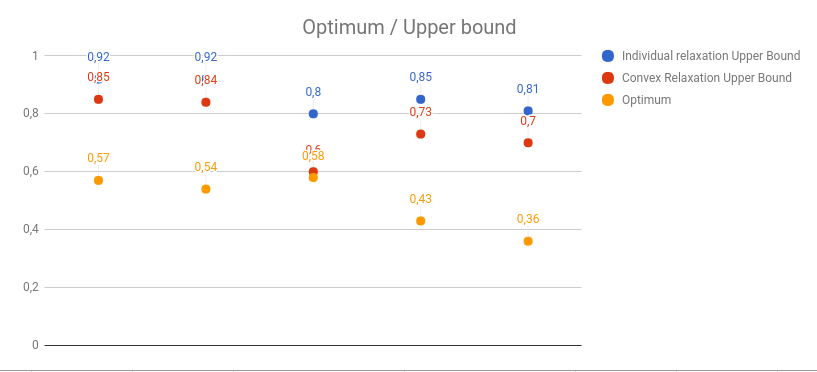
\includegraphics[width=12cm]{media/optimum_upperbound.png}
\end{frame}


\begin{frame}
\begin{itemize}
	\item Individual relaxation upper bound computation is faster
\end{itemize}
\hspace*{-0.8cm}
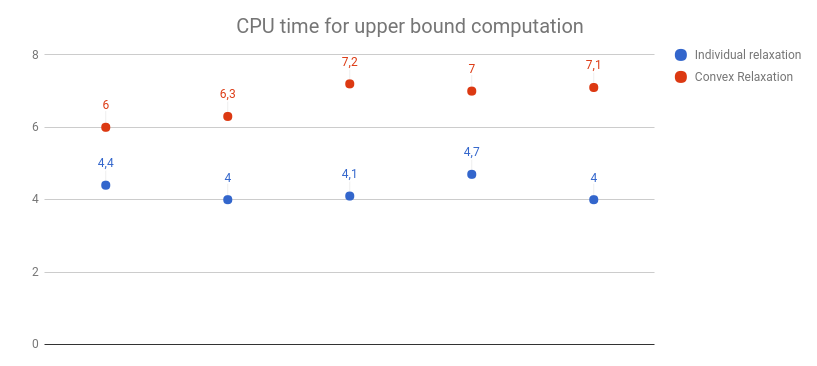
\includegraphics[width=12cm]{media/cpu_upper.png}
\end{frame}
	

\begin{frame}
\begin{itemize}
	\item convex relaxation optimum computation is faster (upper bound is smaller)
\end{itemize}
\hspace*{-0.8cm}
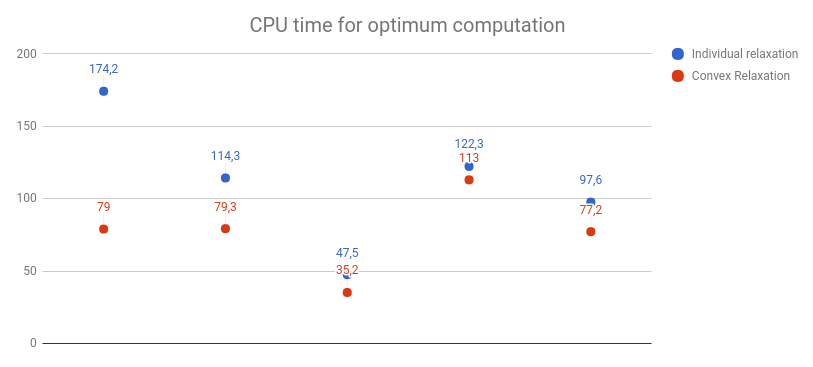
\includegraphics[width=12cm]{media/cpu_opt.png}
\end{frame}

\begin{frame}
	Graphs kind
	\begin{itemize}
		\item \textbf{$(n,m) = (23,40)$ (chart)}.
		\pause
		\item $(n,m) = (50,413)$.
		\pause
		\item random graphs with $n=50$.
	\end{itemize}
	\pause
	Method easily extendable to solve larger size instances.
\end{frame}

\begin{frame}
	\begin{block}{Conclusion}
		\begin{itemize}
			\pause
			\item the paper proposes a branch and bound framework to solve the stochastic resource constrained shortest path 
			\pause
			\item it introduces a convex relaxation to find the upper bound.
			\pause
			\item it shows by experiments that this convex relaxation outperforms indivudal relaxation.
		\end{itemize}
	\end{block}
	\pause
	\begin{block}{Going further}
		\begin{itemize}
			\item generalize to dependent random variable
			\pause
			\item study the influence of some variable (for exemple $N$, the number of segment in tangent approximation, on the CPU time / upper bound value).
			\pause
			\item find a lower bound to give the branch and bound algorithm with another approximation of $F^{-1}(p_0^{k})$.
		\end{itemize}
	\end{block}
\end{frame}
\begin{frame}
	\begin{center}
	\LARGE{Questions ?}
	\end{center}
\end{frame}
\end{document}
